\chapter{Einleitung}
\label{chap:einleitung}
Durch den technischen Fortschritt in den letzten Jahren hat sich der Einsatz von Augmented Reality (AR) und Virtual Reality (VR) in vielen verschiedenen Anwendungsbereichen etabliert.
Die weite Verbreitung von Smartphones ermöglicht die Entwicklungen von AR- und VR-Anwendungen, welche die Sensoren dieser Geräte (Kameras, Gyrosensor, etc.) ausnutzen.
Aber auch unterschiedliche Head-Mounted Displays (HMDs), wie z.B. die \emph{Microsoft HoloLens} \parencite{Microsoft2018} oder die \emph{HTC Vive} \parencite{HTCCorporation2018}, werden zunehmend in Forschung und Industrie eingesetzt.

Ein Bereich, der von dieser Entwicklung beeinflusst wird, ist die Navigation mit Karten.
Früher musste z.B. während der Autofahrt mit Papierkarten navigiert werden.
Mit dem technologischen Fortschritt verbreitete sich der Einsatz von speziellen GPS-Geräten (Global Positioning System), die inzwischen direkt ins Fahrzeug verbaut werden.
Heutzutage verfügen Smartphones über einen eigenen GPS-Sensor und Apps wie \emph{Google Maps} \parencite{GoogleLLC2018} bieten eine entsprechende Software für die Routenplanung, die Suche nach den nächstgelegenen Restaurants, Öffnungszeiten und Preise von Tankstellen und mehr.
Häufig bieten diese Apps auch die Möglichkeit der Navigation für Fußgänger, Radfahrer und sogar öffentliche Verkehrsmittel.

Ein großer Teil der Forschung im Bereich AR/VR befasst sich mit dem Thema, wie virtuelle Navigationshelfer die Reise zwischen zwei Punkten verbessern können.
Darüber hinaus wird in der Industrie bereits versucht, solche Hinweise direkt in die Windschutzscheiben von Fahrzeugen zu integrieren \parencites{Cunningham2017}{Sygic2018}.

\section{Motivation und Ziel der Arbeit}
\label{sec:motivation_ziel}
Die ursprüngliche Idee für diese Masterarbeit stammt aus dem Spiel \emph{Tom Clancy's The Division} (TCTD) \parencite{Ubisoft2018}, in welches das Konzept einer \enquote{Megamap} umsetzt (\autoref{fig:megamap}).
Eine Karte der Umgebung (eine kleine Variante von New York) wird mit relevanten Spielobjekten und Ortsnamen \emph{im Spiel} als AR-Interface um den Charakter herum angezeigt.
Die Karte erlaubt dem Spieler unter anderem, Wegpunkte festzulegen (Navigation), interessante Punkte in der Umgebung anzuzeigen und zu filtern (Exploration) sowie die Ansicht durch Verschieben und Zoomen der Karte anzupassen.
Ebenso werden Missionsziele, andere Charaktere und Events durch Icons in der Karte hervorgehoben.
All diese Informationen sind vom aktuellen Kontext des Spiels abhängig.
Das heißt, es werden nur Informationen angezeigt die für die aktuelle Spielsituation des Spielers relevant sind.
\begin{figure}[bth]
    \centering
    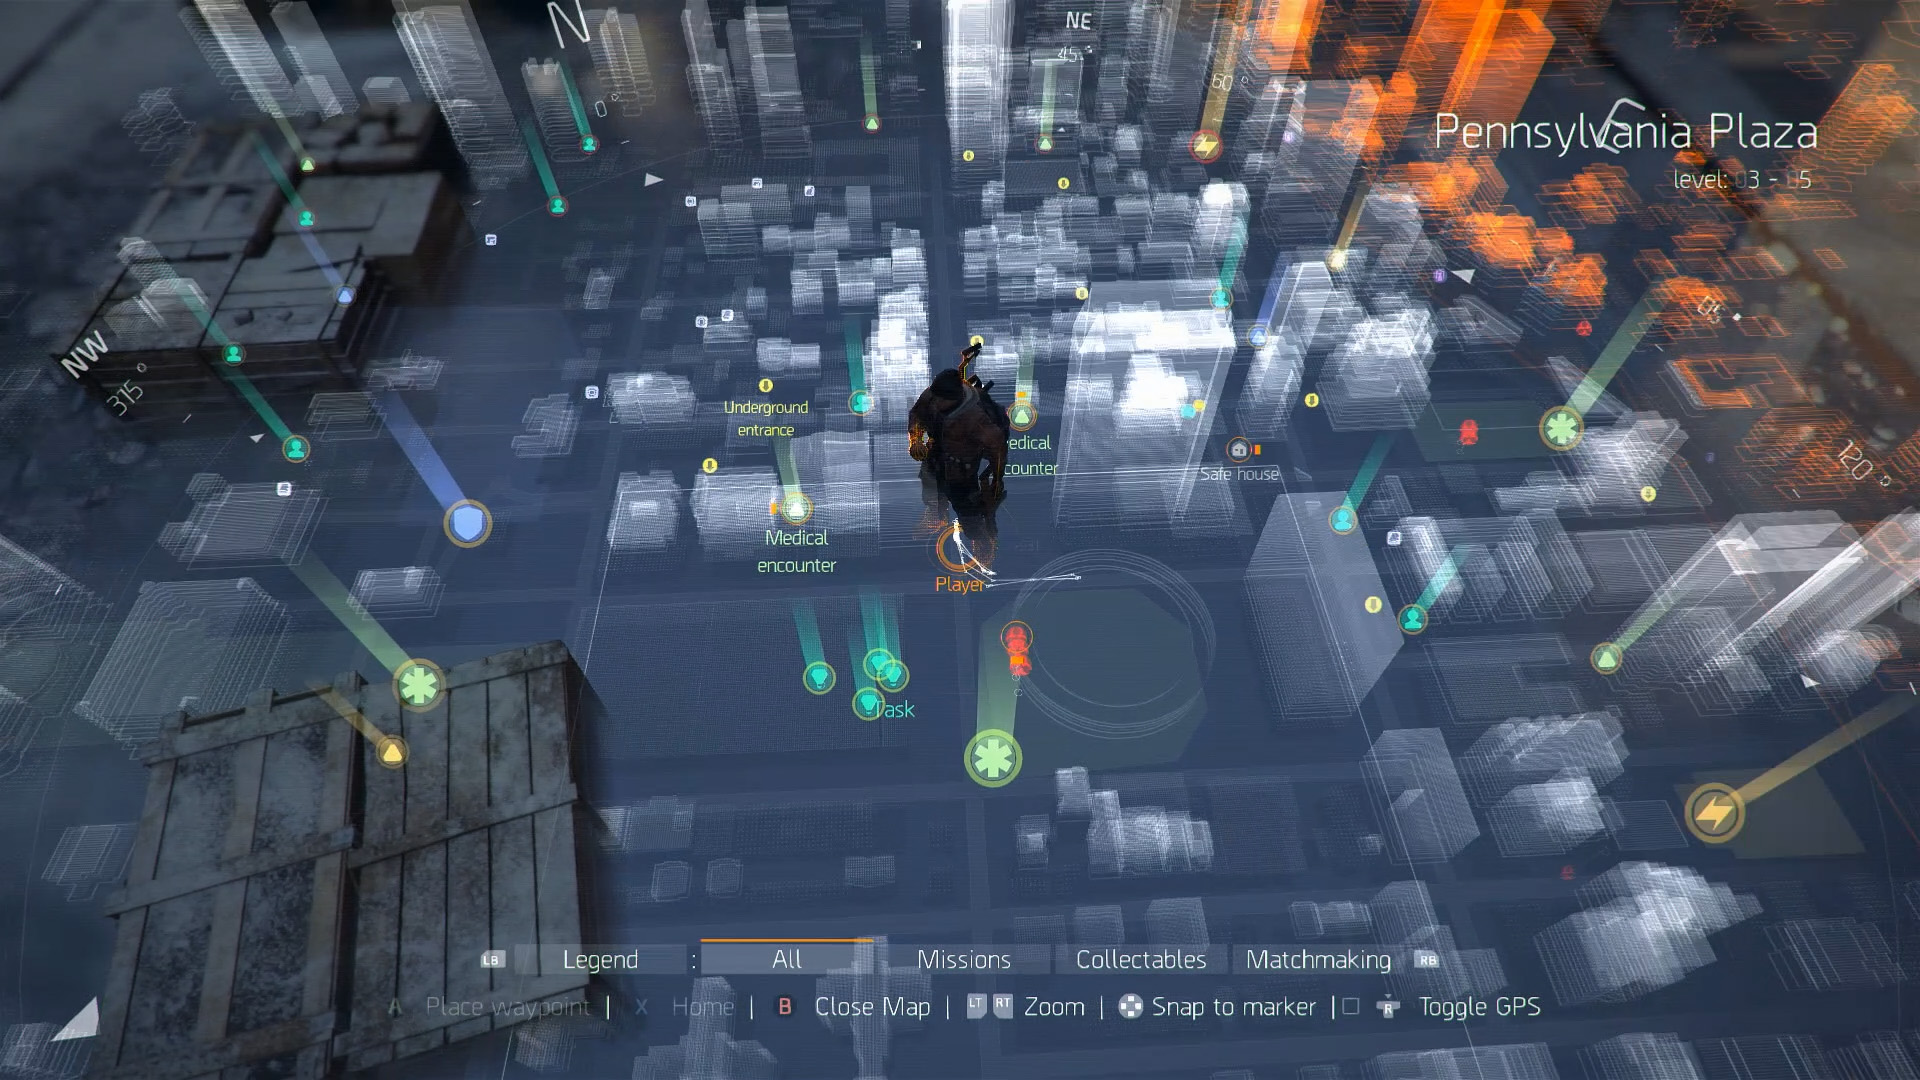
\includegraphics[width=\textwidth]{figures/the_division_megamap.jpg}
    \quelle{\cite{MYDIVISION.NET2014}}
    \caption{Die \enquote{Megamap} aus \emph{Tom Clancy's The Division}. Symbole zeigen Missionsziele, Gegenstände und wichtige Orte im Spiel.}
    \label{fig:megamap}
\end{figure}

Eine Kartendarstellung existiert in dieser Form bisher nur im Spiel.
In der realen Welt werden Karten zwar zunehmend durch AR/VR unterstützt.
Eine Anwendung wie die Megamap aus TCTD, bei der die Karte in die Umgebung integriert ist, gibt es bisher aber noch nicht.
Dafür gibt es mehrere Gründe:
\begin{enumerate}
    \item Die bisherigen Lösungen zur AR-unterstützten Kartenexploration stützen sich meistens auf die Überlagerung von virtuellen Information auf physische Objekte, beispielsweise eine reale Karte.
    Dabei wird häufig ein Smartphone als \emph{Magic Lens} (\enquote{Magische Lupe},~\cite{Bier1994}) eingesetzt, auf dem die virtuellen Informationen vor dem Hintergrund der Kamera angezeigt werden.
    Solch ein Ansatz ist jedoch nur Bedingt für den mobilen Einsatz geeignet.
    Einem Fußgänger würde das gleichzeitige Halten einer Karte und eines Smartphones schwerfallen, besonders während des Laufens.
    Auch der Einsatz eines Projektors, der die Informationen auf eine Karte projiziert, ist hierfür nicht geeignet.

    \item Die durch virtuelle Helfer unterstützte Navigation ist ein Ansatz, der sich in der Forschung häufig finden lässt.
    Allerdings ist die reine Navigation nicht der einzige Anwendungsfall in Bezug auf Kartenanwendungen.
    Wie \textcite{Reichenbacher2001} detailliert beschreibt gibt es weitere Anwendungsfälle, die sich unter dem Oberbegriff der \emph{Kartenexploration} zusammenfassen lassen.
    Darin eingeschlossen sind zum Beispiel die zuvor erwähnten Szenarios der Restaurantsuche oder der Anzeige von Fahrt- oder Öffnungszeiten.
    Allgemein gesagt geht es bei der Kartenexploration um die \enquote{Entdeckung} von Orten anhand von Karten.
    Diese Anwendungsfälle werden jedoch, in Bezug auf Unterstützung durch AR/VR, seltener behandelt als die Unterstützung der reinen Navigation.

    \item Die bisherigen Ansätze stützen sich meistens auf den Einsatz von Smartphones oder anderen Handgeräten.
    Obwohl die Entwicklung dieser Geräte technologisch rasch voranschreitet, sind sie auf die Möglichkeiten der Kamera-Bildsensoren, Gyrosensoren und GPS-Sensoren beschränkt.
    Z.B. ist die dreidimensionale Rekonstruktion einer Szene, wenn überhaupt, nur sehr vereinfacht möglich.
\end{enumerate}

Die Integration der Karte in die Umgebung wäre jedoch von Vorteil.
Denn eine von der Umgebung getrennte virtuelle Karte, wie es bei vielen aktuellen Smartphone-Anwendungen der Fall ist, kann die Aufmerksamkeit des Nutzers von der eigentlichen Umgebung ablenken.
Die Nutzer müssen ständig das virtuelle Bild mit ihrer Umgebung abgleichen.
Dies ist nicht nur ein zusätzlicher mentaler Aufwand.
Im schlimmsten Fall kann es zu schweren Unfällen kommen wenn die Nutzer auf die virtuelle Darstellung achten oder die dargestellten Informationen beim Abgleich mit der Umgebung fehlinterpretieren \parencites{Medenica2011}{Lin2017}.

Weitere Schwierigkeiten ergeben sich bei der Darstellung von \emph{Indoor}-Karten (Karten von Gebäuden).
Die Überlagerung von mehreren Stockwerken stellt ebenso ein Problem dar wie die Tatsache, dass das GPS innerhalb von Gebäuden nicht verfügbar ist.
Daher setzen sich viele existierende Ansätze mit der \emph{Navigation} oder Lokalisierung innerhalb von Gebäuden auseinander.
Der Anwendungsfall der Karten\emph{exploration} von Gebäuden wird hingegen bisher kaum behandelt.
Weil kaum öffentliche Gebäudedaten verfügbar sind (im Gegensatz zu \emph{Outdoor}-Daten wie z.B. von \emph{Open Street Map}) wird die Situation weiter erschwert.

Auf die gennanten Probleme wird in dieser Masterarbeit eingegangen.
Zu diesem Zweck wird eine Indoor-Megamap-Kartenanwendung für den Anwendungsfall der Kartenexploration entwickelt.
Hierfür werden öffentlich verfügbare Gebäudedaten genutzt, um eine 3D-Indoor-Repräsentation eines Gebäudes zu erstellen.
Die 3D-Indoor-Karte wird dann in einer virtuellen Umgebung platziert.
Nutzer können dann über virtuelle Bedienelemente mit der Karte interagieren.
Insbesodnere stehen verschiedene explorative Funktionen bereit, beispielsweise das Suchen nach den Büros von Personen oder den Standorten von öffentlichen Druckern.
Nutzer können sich mit der Megamap einen detaillierten Überblick über das Gebäude verschaffen, in dem sie sich befinden.

Als Zielplattform dient das Vive-HMD.
HMDs haben gegenüber Smartphones einige technische Vorteile.
Positionen und Orientierungen der Nutzer sind über Tracking präziser möglich.
\emph{Mixed Reality}-HMDs (MR-HMDs) wie die HoloLens oder die \emph{Magic Leap One} \parencite{MagicLeap2018} verwenden Infrarotkameras, um Strukturen der Umgebung virtuell in Echzeit zu rekonstruieren.
Die reale Umgebung bleibt dank des durchsichtigen Glases weiterhin sichtbar.
Zudem können die Hände für Gesteninteraktionen oder Kontroller verwendet werden anstatt das Display halten zu müssen.

Die ursprüngliche Idee war die Implementierung der Megamap für das Magic Leap One HMD.
Da dieses aber zum Zeitpunkt des Verfassens der Arbeit nicht öffentlich verfügbar ist, wird die Implementierung für das Vive-HMD in VR umgesetzt.
Die \enquote{reale} Umgebung des Nutzers wird dabei virtuell nachgebildet.
Dadurch lässt sich die in dieser Arbeit entwickelte Anwendung später auf ein MR-HMD übertragen.

Die Implementierung der Megamap dient der Beantwortung der zentralen Fragestellung dieser Arbeit:
\begin{quote}
    \itshape
    Ist eine in die Umgebung integrierte 3D-Megamap geeignet, um Nutzer bei der Exploration von Gebäuden zu unterstützen?
\end{quote}
Der Prototyp wird daher in einer Nutztungsevaluation getestet, um seine Effektivität für die Gebäudeexploration festzustellen.

Als Inspirationsquelle für die Anwendung dienen neben bereits existierenden Kartenanwendungen wie Google Maps und Ansätzen aus der Forschung auch digitale Spiele.
Da in Spielen Aufgaben wie Navigation und Exploration von großer Bedeutung sind, kann hier unterschiedliche Ansätze zur Navigations- und Explorationsunterstützung gefunden werden.
Dies ist am Beispiel TCTD erkennbar.

\section{Struktur der Arbeit}
\label{sec:struktur}
Weitergehend ist diese Arbeit in die folgenden Abschnitte unterteilt:

Im nächsten Kapitel wird der Stand der Forschung und Technik zur Darstellung von dreidimensionalen Karten beleuchtet.
Die Unterschiede zum Konzept dieser Arbeit sowie deren Beitrag zum Thema werden ebenso herausgearbeitet.

\autoref{chap:concept} geht detailliert auf die Konzeptionierung der 3D-Megamap ein.
Es wird vor allem beschrieben, welche Interaktionen für die Kartenexploration wichtig sind und wie diese in der Megamap-Anwendung umgesetzt werden sollen.

Danach wird in \autoref{chap:implementation} die Implementierung der Anwendung beschrieben.
Ebenso werden Probleme bei der Implementierung erläutert, die für zukünftige Arbeiten beachtet werden sollten.

\autoref{chap:evaluation} präsentiert die Durchführung der Nutzungsevaluation der Anwendung sowie deren Ergebnisse.
Der Mehrwert der 3D-Megamap im Vergleich zu bisherigen Ansätzen wird ebenfalls diskutiert.

Schließlich werden in \autoref{chap:closing} offene Fragen und Probleme dieser Arbeit genannt, welche für zukünftige Arbeiten von Interesse sind.
% TODO Ist das wirklich eine Einschätzung?
Ebenso wird das Potential von 3D-Karten in Kombination mit anderen, nicht in dieser Arbeit behandelten Technologien eingeschätzt.
%
\cleardoublepage
